\documentclass[border=6pt]{standalone}
\usepackage{amsmath}
\usepackage{amssymb}
\usepackage{tikz}
\usepackage{pgfplots}
\pgfplotsset{compat=1.18}
\usetikzlibrary{arrows.meta,calc,positioning}
\begin{document}
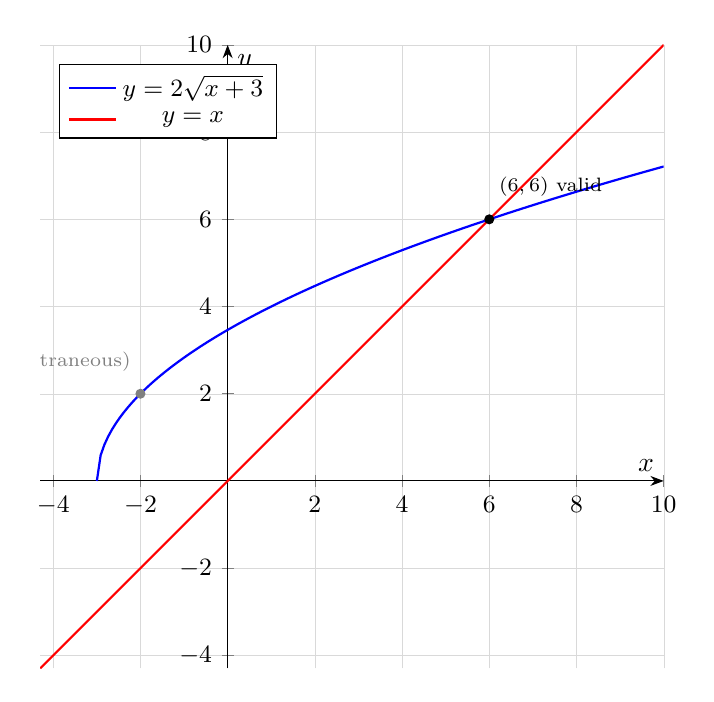
\begin{tikzpicture}
\begin{axis}[
    axis lines = middle,
    xlabel = {$x$}, ylabel = {$y$},
    grid=both,
    grid style={line width=.1pt, draw=gray!30},
    axis line style={-Stealth},
    legend style={font=\small},
    tick label style={font=\small},
    xmin=-4.3, xmax=10, ymin=-4.3, ymax=10,
    xtick={-4,-2,0,2,4,6,8,10},
    ytick={-4,-2,0,2,4,6,8,10},
    width=9.5cm, height=9.5cm,
    legend pos=north west,
]
\addplot[domain=-3:10, samples=150, thick, blue] {2*sqrt(x+3)};
\addlegendentry{$y=2\sqrt{x+3}$}
\addplot[domain=-4.3:10, samples=2, thick, red] {x};
\addlegendentry{$y=x$}
\addplot[only marks, mark=*, mark size=1.6pt, black] coordinates {(6,6)};
\node[anchor=south west, font=\scriptsize] at (axis cs:6,6.3) {$(6,6)$ valid};
\addplot[only marks, mark=*, mark size=1.6pt, gray] coordinates {(-2,2)};
\node[anchor=south east, font=\scriptsize, gray] at (axis cs:-2,2.3) {$(-2,2)$ (extraneous)};
\end{axis}
\end{tikzpicture}
\end{document}
